\hypertarget{group__genetic}{
\section{Genetico}
\label{group__genetic}\index{Genetico@{Genetico}}
}


\subsection{Descripci\'{o}n detallada}
Dentro del modulo genetico encontraremos una implementacion de heuristicas de algoritmos geneticos y evoluticos que seleccionara la solucion. 

\subsection*{Archivos}
\begin{CompactItemize}
\item 
archivo \hyperlink{genesting_8h}{genesting.h}
\item 
archivo \hyperlink{individuo_8h}{individuo.h}
\item 
archivo \hyperlink{population_8h}{population.h}
\item 
archivo \hyperlink{genesting_8c}{genesting.c}
\item 
archivo \hyperlink{individuo_8c}{individuo.c}
\item 
archivo \hyperlink{population_8c}{population.c}
\end{CompactItemize}
\subsection*{Clases}
\begin{CompactItemize}
\item 
struct \hyperlink{struct__genesting}{\_\-genesting}
\item 
struct \hyperlink{struct__posicion}{\_\-posicion}
\item 
struct \hyperlink{struct__individuo}{\_\-individuo}
\item 
struct \hyperlink{struct__population}{\_\-population}
\end{CompactItemize}
\subsection*{Tipos definidos}
\begin{CompactItemize}
\item 
typedef \hyperlink{struct__genesting}{\_\-genesting} \hyperlink{group__genetic_gcd77cefe71c44c38745a4f148c7a69eb_gcd77cefe71c44c38745a4f148c7a69eb}{genesting}
\item 
typedef \hyperlink{struct__posicion}{\_\-posicion} \hyperlink{group__genetic_ge2fa8f912ec24aab702abf9b76489462_ge2fa8f912ec24aab702abf9b76489462}{posicion}
\item 
typedef \hyperlink{struct__individuo}{\_\-individuo} \hyperlink{group__genetic_g86fcc12a3e2577bedca3b8364e722da3_g86fcc12a3e2577bedca3b8364e722da3}{individuo}
\item 
typedef \hyperlink{struct__population}{\_\-population} \hyperlink{group__genetic_gdc93697b2d7197da72db59932b540a07_gdc93697b2d7197da72db59932b540a07}{population}
\end{CompactItemize}
\subsection*{Funciones}
\begin{CompactItemize}
\item 
\hyperlink{struct__genesting}{genesting} $\ast$ \hyperlink{group__genetic_g6fed4910dd1f6172bb5a4e35a97bbe56_g6fed4910dd1f6172bb5a4e35a97bbe56}{leer\_\-archivo} (char $\ast$arc\_\-name)
\item 
void \hyperlink{group__genetic_g1daa6a4e8af34b8b16a48fc2f3701f1c_g1daa6a4e8af34b8b16a48fc2f3701f1c}{genesting\_\-init} (\hyperlink{struct__genesting}{genesting} $\ast$g)
\item 
void \hyperlink{group__genetic_g3f63f4034274d731cb3fdf3200c64d41_g3f63f4034274d731cb3fdf3200c64d41}{genesting\_\-show} (\hyperlink{struct__genesting}{genesting} $\ast$g)
\item 
float \hyperlink{group__genetic_gf152bd4602acec2166cc4b91e8c8919a_gf152bd4602acec2166cc4b91e8c8919a}{individuo\_\-fitness} (\hyperlink{struct__individuo}{individuo} $\ast$ind)
\item 
void \hyperlink{group__genetic_gf4e60223d27c85a5f6166e35ecafe641_gf4e60223d27c85a5f6166e35ecafe641}{individuo\_\-create} (\hyperlink{struct__genesting}{genesting} $\ast$g, \hyperlink{struct__individuo}{individuo} $\ast$ind)
\item 
void \hyperlink{group__genetic_g05b6d3d7a4be17c9cbf479f424edd01b_g05b6d3d7a4be17c9cbf479f424edd01b}{individuo\_\-mutate} (\hyperlink{struct__individuo}{individuo} $\ast$ind)
\item 
void \hyperlink{group__genetic_g18105662f4835e24cf3b8fc40ed63b33_g18105662f4835e24cf3b8fc40ed63b33}{individuo\_\-procreate} (\hyperlink{struct__individuo}{individuo} $\ast$p, \hyperlink{struct__individuo}{individuo} $\ast$m, \hyperlink{struct__individuo}{individuo} $\ast$ind)
\item 
bool \hyperlink{group__genetic_gf80cc38ea4d590f6c45215f770d63778_gf80cc38ea4d590f6c45215f770d63778}{individuo\_\-validate} (\hyperlink{struct__individuo}{individuo} $\ast$ind)
\item 
int \hyperlink{group__genetic_gd9507b892f115e76cd4162059839370c_gd9507b892f115e76cd4162059839370c}{comparar\_\-individuos} (\hyperlink{struct__individuo}{individuo} $\ast$ind1, \hyperlink{struct__individuo}{individuo} $\ast$ind2)
\item 
void \hyperlink{group__genetic_gc7ba874876f18abab66f0a42f32b98cc_gc7ba874876f18abab66f0a42f32b98cc}{population\_\-create} (\hyperlink{struct__population}{population} $\ast$p, \hyperlink{struct__genesting}{genesting} $\ast$g, int n)
\item 
void \hyperlink{group__genetic_g229293c432c5ef4f70b1ee94c109bb1a_g229293c432c5ef4f70b1ee94c109bb1a}{population\_\-evaluate} (\hyperlink{struct__population}{population} $\ast$p)
\item 
void \hyperlink{group__genetic_g5b3202f02e14d7fb3eb1f729d1250243_g5b3202f02e14d7fb3eb1f729d1250243}{population\_\-generation} (\hyperlink{struct__population}{population} $\ast$p)
\end{CompactItemize}


\subsection{Documentaci\'{o}n de los tipos definidos}
\hypertarget{group__genetic_gcd77cefe71c44c38745a4f148c7a69eb_gcd77cefe71c44c38745a4f148c7a69eb}{
\index{genetic@{genetic}!genesting@{genesting}}
\index{genesting@{genesting}!genetic@{genetic}}
\subsubsection[genesting]{\setlength{\rightskip}{0pt plus 5cm}typedef struct \hyperlink{struct__genesting}{\_\-genesting} \hyperlink{struct__genesting}{genesting}}}
\label{group__genetic_gcd77cefe71c44c38745a4f148c7a69eb_gcd77cefe71c44c38745a4f148c7a69eb}




Definici\'{o}n en la l\'{\i}nea 25 del archivo genesting.h.\hypertarget{group__genetic_g86fcc12a3e2577bedca3b8364e722da3_g86fcc12a3e2577bedca3b8364e722da3}{
\index{genetic@{genetic}!individuo@{individuo}}
\index{individuo@{individuo}!genetic@{genetic}}
\subsubsection[individuo]{\setlength{\rightskip}{0pt plus 5cm}typedef struct \hyperlink{struct__individuo}{\_\-individuo} \hyperlink{struct__individuo}{individuo}}}
\label{group__genetic_g86fcc12a3e2577bedca3b8364e722da3_g86fcc12a3e2577bedca3b8364e722da3}




Definici\'{o}n en la l\'{\i}nea 19 del archivo individuo.h.\hypertarget{group__genetic_gdc93697b2d7197da72db59932b540a07_gdc93697b2d7197da72db59932b540a07}{
\index{genetic@{genetic}!population@{population}}
\index{population@{population}!genetic@{genetic}}
\subsubsection[population]{\setlength{\rightskip}{0pt plus 5cm}typedef struct \hyperlink{struct__population}{\_\-population} \hyperlink{struct__population}{population}}}
\label{group__genetic_gdc93697b2d7197da72db59932b540a07_gdc93697b2d7197da72db59932b540a07}




Definici\'{o}n en la l\'{\i}nea 21 del archivo population.h.\hypertarget{group__genetic_ge2fa8f912ec24aab702abf9b76489462_ge2fa8f912ec24aab702abf9b76489462}{
\index{genetic@{genetic}!posicion@{posicion}}
\index{posicion@{posicion}!genetic@{genetic}}
\subsubsection[posicion]{\setlength{\rightskip}{0pt plus 5cm}typedef struct \hyperlink{struct__posicion}{\_\-posicion} \hyperlink{struct__posicion}{posicion}}}
\label{group__genetic_ge2fa8f912ec24aab702abf9b76489462_ge2fa8f912ec24aab702abf9b76489462}




Definici\'{o}n en la l\'{\i}nea 17 del archivo individuo.h.

\subsection{Documentaci\'{o}n de las funciones}
\hypertarget{group__genetic_gd9507b892f115e76cd4162059839370c_gd9507b892f115e76cd4162059839370c}{
\index{genetic@{genetic}!comparar_individuos@{comparar\_\-individuos}}
\index{comparar_individuos@{comparar\_\-individuos}!genetic@{genetic}}
\subsubsection[comparar\_\-individuos]{\setlength{\rightskip}{0pt plus 5cm}int comparar\_\-individuos (\hyperlink{struct__individuo}{individuo} $\ast$ {\em ind1}, \hyperlink{struct__individuo}{individuo} $\ast$ {\em ind2})}}
\label{group__genetic_gd9507b892f115e76cd4162059839370c_gd9507b892f115e76cd4162059839370c}


Compara entre los dos individuos cual es mejor segun su fitness 

Definici\'{o}n en la l\'{\i}nea 275 del archivo individuo.c.

\begin{Code}\begin{verbatim}276 {
277     return ((int)(((ind1->fitness)-(ind2->fitness))*10000.0));
278 }
\end{verbatim}\end{Code}


\hypertarget{group__genetic_g1daa6a4e8af34b8b16a48fc2f3701f1c_g1daa6a4e8af34b8b16a48fc2f3701f1c}{
\index{genetic@{genetic}!genesting_init@{genesting\_\-init}}
\index{genesting_init@{genesting\_\-init}!genetic@{genetic}}
\subsubsection[genesting\_\-init]{\setlength{\rightskip}{0pt plus 5cm}void genesting\_\-init (\hyperlink{struct__genesting}{genesting} $\ast$ {\em g})}}
\label{group__genetic_g1daa6a4e8af34b8b16a48fc2f3701f1c_g1daa6a4e8af34b8b16a48fc2f3701f1c}


Realiza unas correcciones iniciales al archivo de entrada y calcula los valores fijos del problema, como el area maxima y volumen maximo que se dan cuando generamos una solucion vacia. 

Definici\'{o}n en la l\'{\i}nea 87 del archivo genesting.c.

\begin{Code}\begin{verbatim}88 {
89     int i;
90     float minx, miny, maxx, maxy;
91     polygon_holes p;
92 
93     polygon_minbox(&(g->plantilla), &minx, &miny, &maxx, &maxy);
94 
95     polygon_translate(&(g->plantilla), -minx, -miny);
96 
97     for (i=0;i<g->nhuecos;i++)
98     {
99         polygon_translate(&(g->huecos[i]), -minx, -miny);
100     }
101 
102     for (i=0;i<g->npatrones;i++)
103     {
104         polygon_minbox(&(g->patrones[i]), &minx, &miny, &maxx, &maxy);
105         polygon_translate(&(g->patrones[i]), -minx, -miny);
106     }
107 
108     p.nholes = g->nhuecos;
109     p.p = &(g->plantilla);
110     p.h = g->huecos;
111 
112     g->area = polygonholes_area(&p);
113 
114     g->volumen = polygonholes_volumen(&p);
115 }
\end{verbatim}\end{Code}




Gr\'{a}fico de llamadas para esta funci\'{o}n:\begin{figure}[H]
\begin{center}
\leavevmode
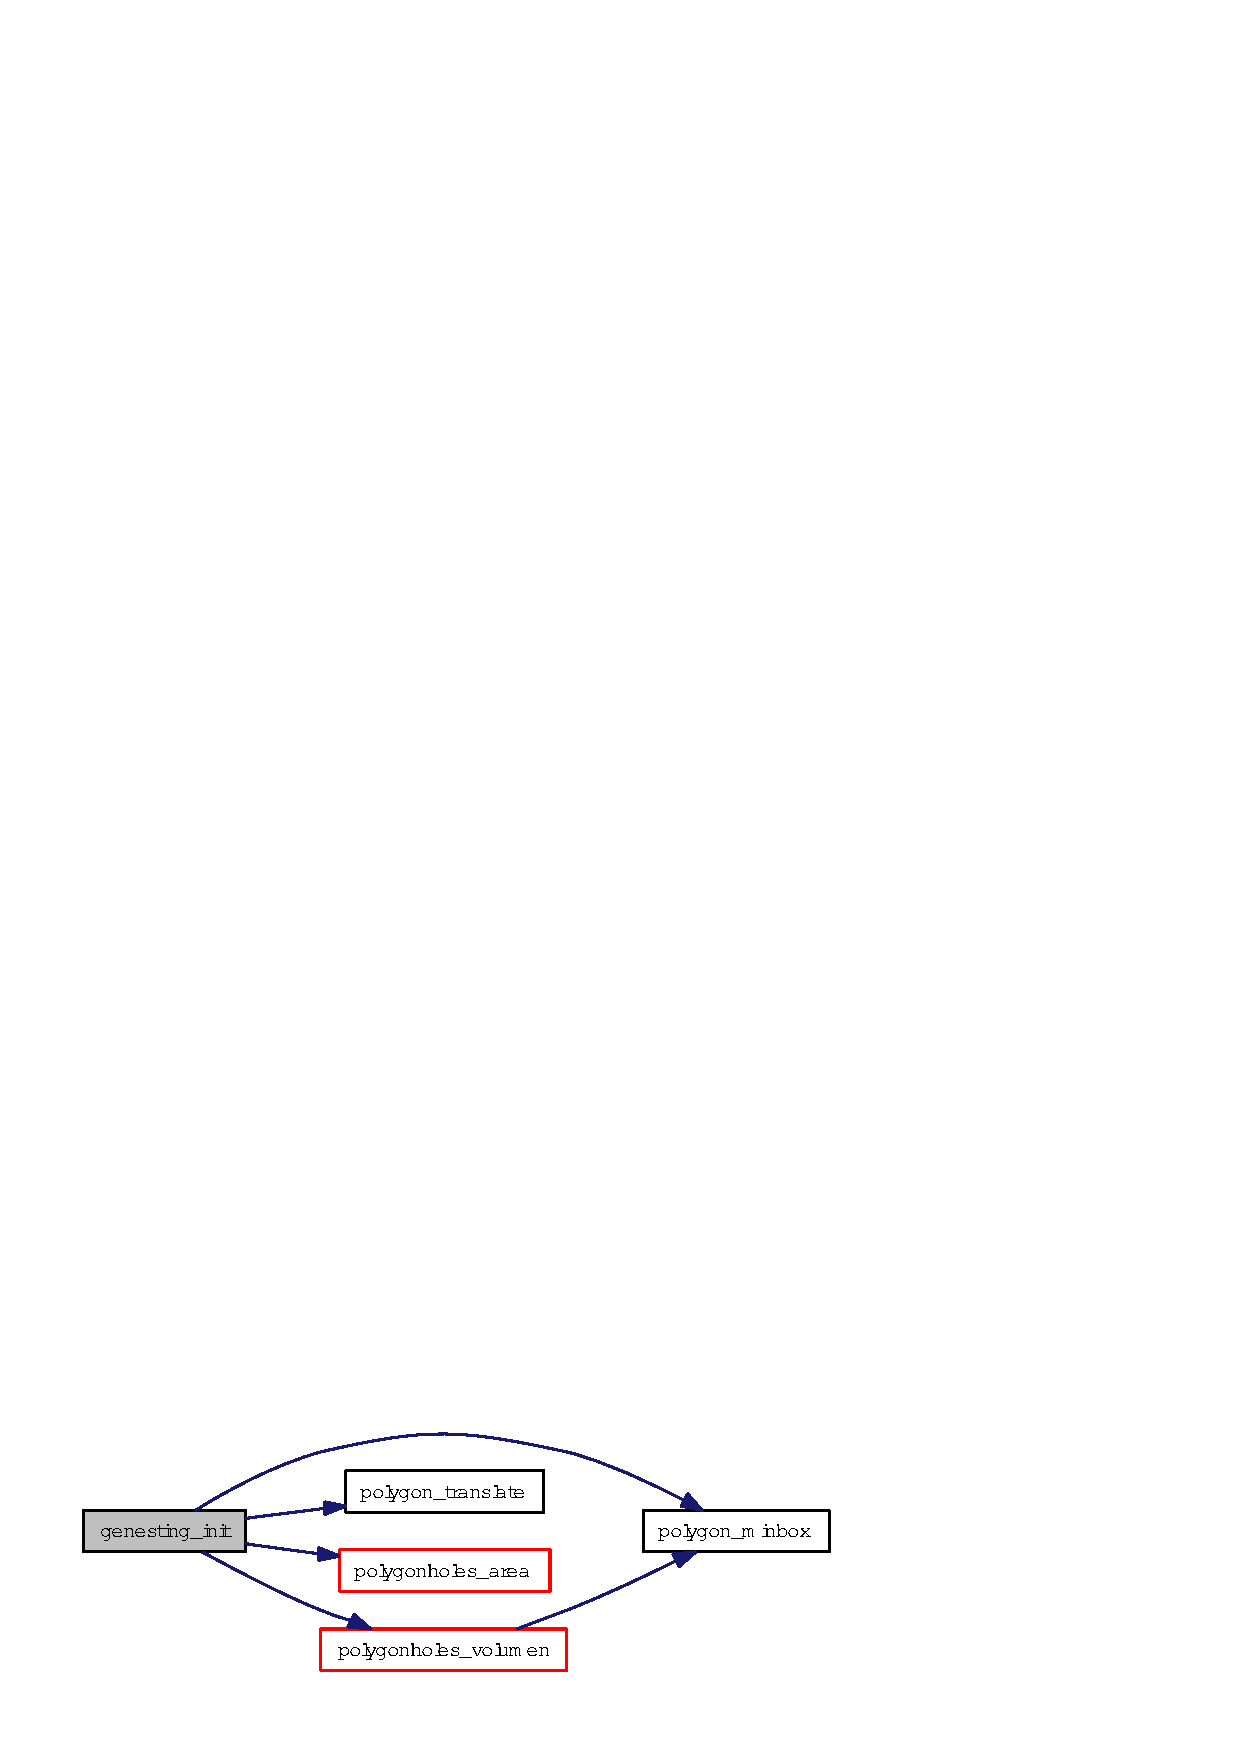
\includegraphics[width=201pt]{group__genetic_g1daa6a4e8af34b8b16a48fc2f3701f1c_g1daa6a4e8af34b8b16a48fc2f3701f1c_cgraph}
\end{center}
\end{figure}


Here is the caller graph for this function:\begin{figure}[H]
\begin{center}
\leavevmode
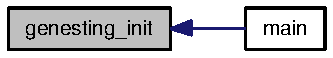
\includegraphics[width=98pt]{group__genetic_g1daa6a4e8af34b8b16a48fc2f3701f1c_g1daa6a4e8af34b8b16a48fc2f3701f1c_icgraph}
\end{center}
\end{figure}
\hypertarget{group__genetic_g3f63f4034274d731cb3fdf3200c64d41_g3f63f4034274d731cb3fdf3200c64d41}{
\index{genetic@{genetic}!genesting_show@{genesting\_\-show}}
\index{genesting_show@{genesting\_\-show}!genetic@{genetic}}
\subsubsection[genesting\_\-show]{\setlength{\rightskip}{0pt plus 5cm}void genesting\_\-show (\hyperlink{struct__genesting}{genesting} $\ast$ {\em g})}}
\label{group__genetic_g3f63f4034274d731cb3fdf3200c64d41_g3f63f4034274d731cb3fdf3200c64d41}


Muestra la informacion del programa \begin{Desc}
\item[Par\'{a}metros:]
\begin{description}
\item[\mbox{$\leftarrow$} {\em g}]Genesting \end{description}
\end{Desc}


Definici\'{o}n en la l\'{\i}nea 121 del archivo genesting.c.

\begin{Code}\begin{verbatim}122 {
123     int i;
124 
125     printf("Mostrando informacion de genesting\n");
126     printf("Plantilla:\n");
127     printf("  Vertices: %i\n",g->plantilla.nvertices);
128     printf("  Area: %f\n",polygon_area(&(g->plantilla)));
129 
130     printf("Huecos: %i\n",g->nhuecos);
131     for (i=0;i<g->nhuecos;i++)
132     {
133         printf("  Hueco %i:\n",i+1);
134         printf("    Vertices: %i\n",g->huecos[i].nvertices);
135         printf("    Area: %f\n",polygon_area(&(g->huecos[i])));
136     }
137 
138     printf("Area Util: %f\n",g->area);
139     printf("Volumen Util: %f\n",g->volumen);
140 
141     printf("Patrones: %i\n",g->npatrones);
142     for (i=0;i<g->npatrones;i++)
143     {
144         printf("  Patrones %i:\n",i+1);
145         printf("    Vertices: %i\n",g->patrones[i].nvertices);
146         printf("    Area: %f\n",polygon_area(&(g->patrones[i])));
147     }
148 }
\end{verbatim}\end{Code}




Gr\'{a}fico de llamadas para esta funci\'{o}n:\begin{figure}[H]
\begin{center}
\leavevmode
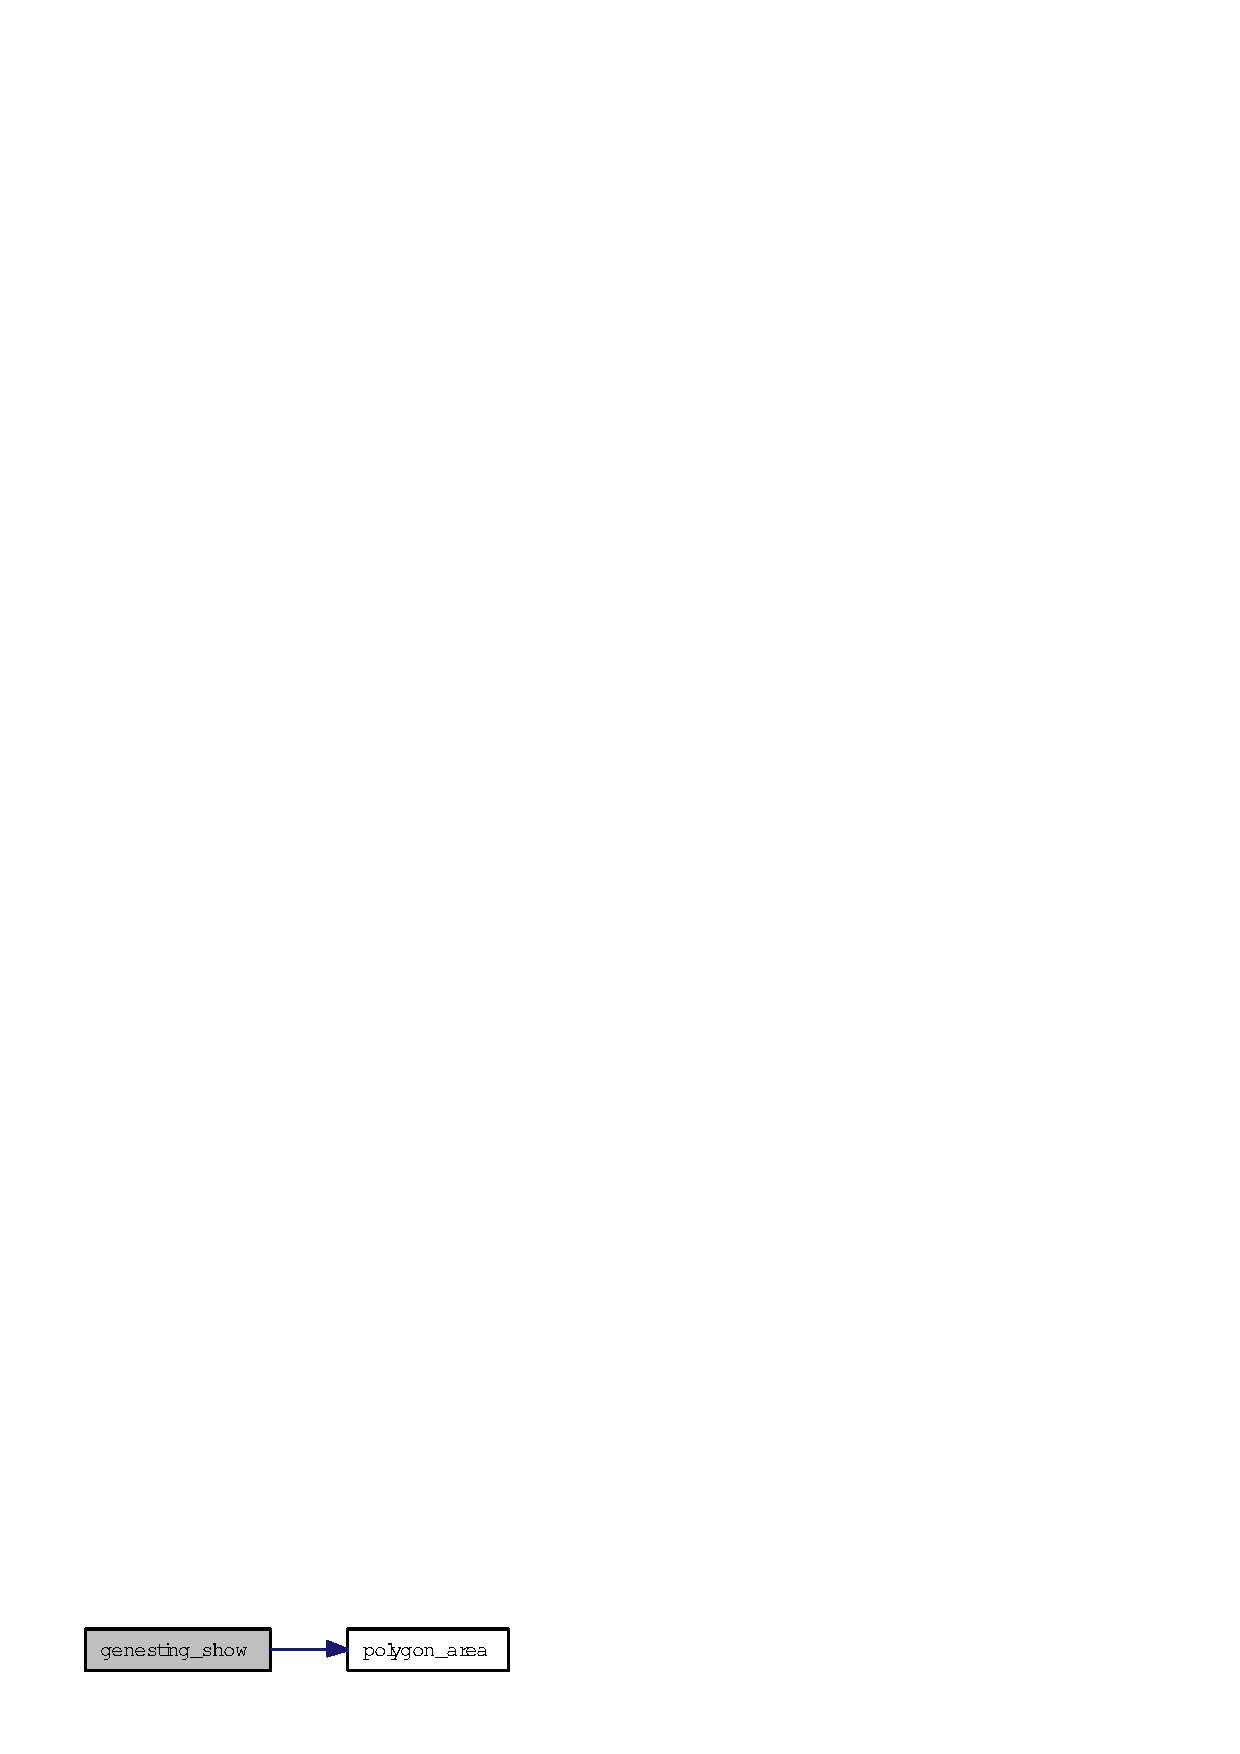
\includegraphics[width=124pt]{group__genetic_g3f63f4034274d731cb3fdf3200c64d41_g3f63f4034274d731cb3fdf3200c64d41_cgraph}
\end{center}
\end{figure}


Here is the caller graph for this function:\begin{figure}[H]
\begin{center}
\leavevmode
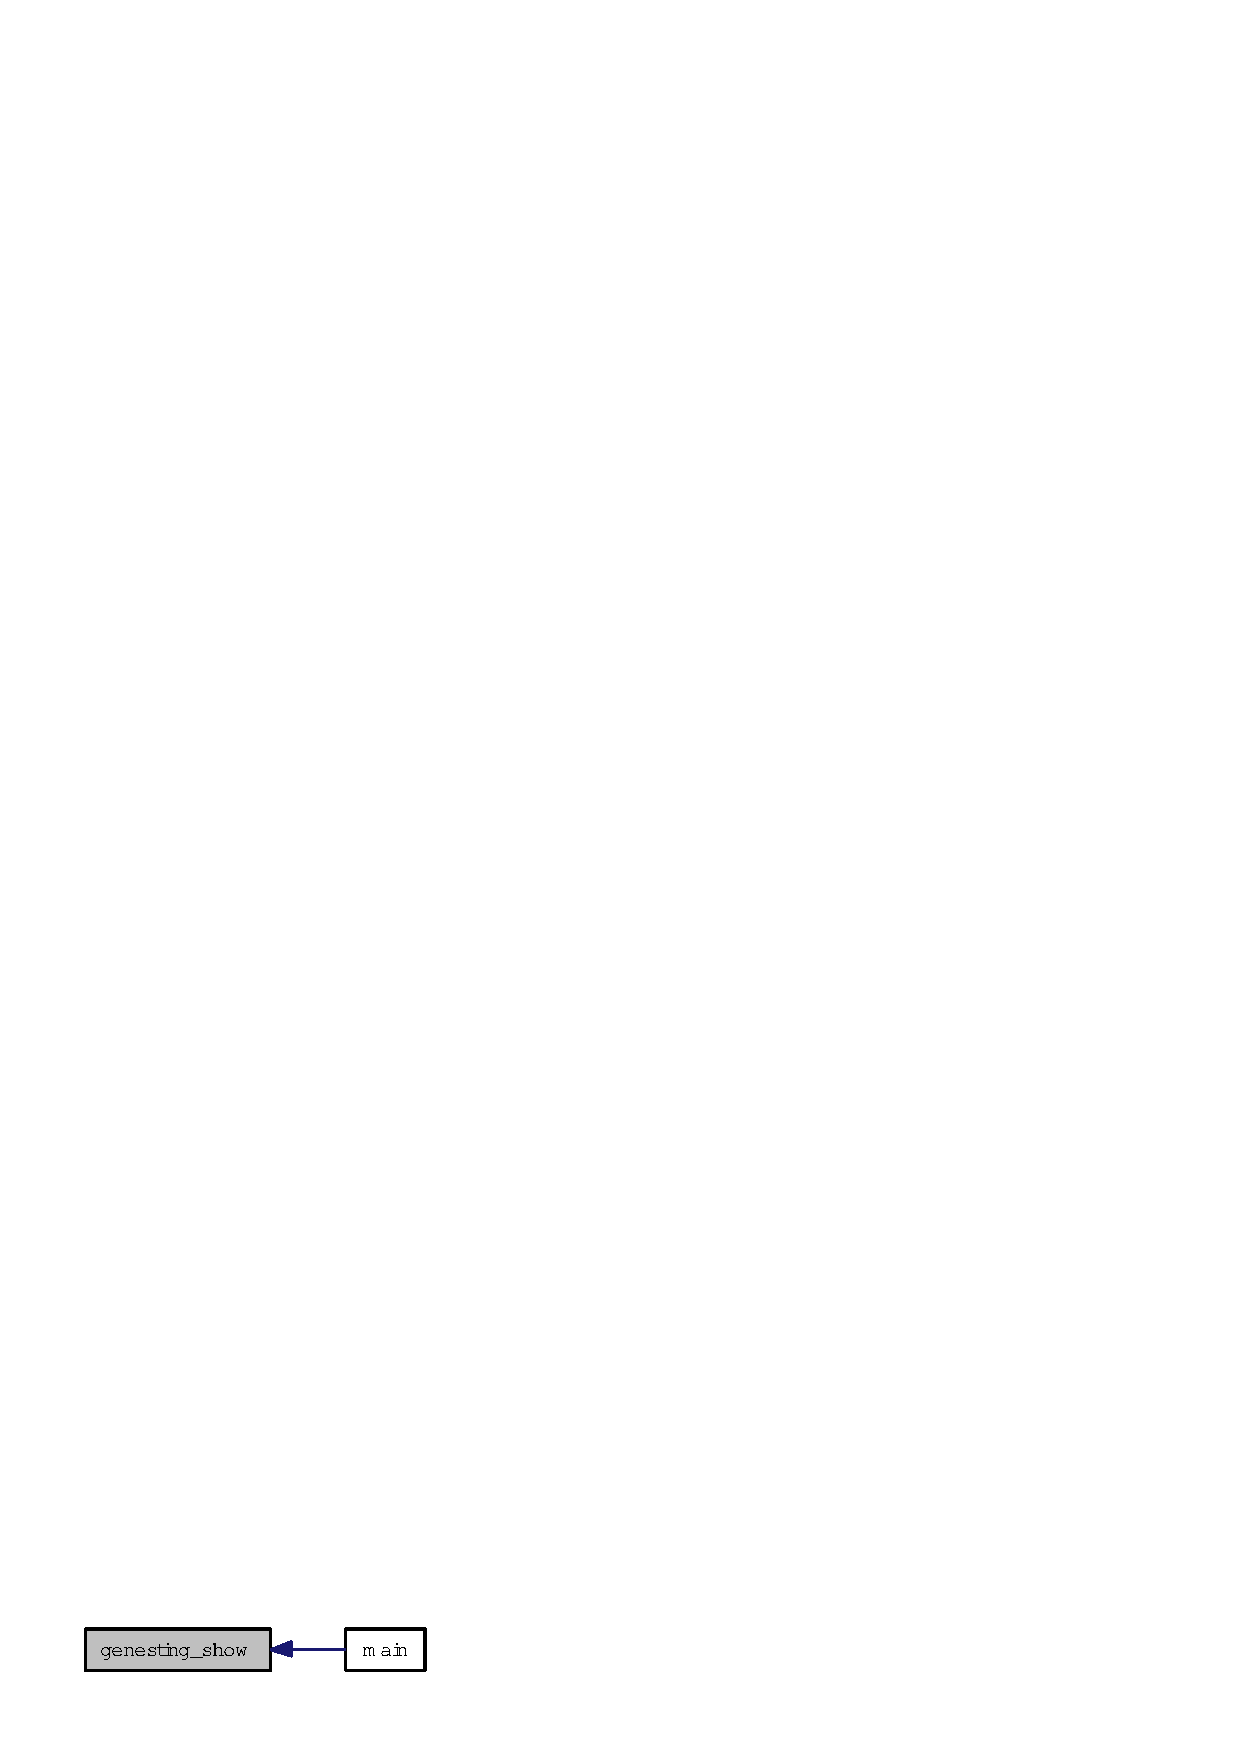
\includegraphics[width=104pt]{group__genetic_g3f63f4034274d731cb3fdf3200c64d41_g3f63f4034274d731cb3fdf3200c64d41_icgraph}
\end{center}
\end{figure}
\hypertarget{group__genetic_gf4e60223d27c85a5f6166e35ecafe641_gf4e60223d27c85a5f6166e35ecafe641}{
\index{genetic@{genetic}!individuo_create@{individuo\_\-create}}
\index{individuo_create@{individuo\_\-create}!genetic@{genetic}}
\subsubsection[individuo\_\-create]{\setlength{\rightskip}{0pt plus 5cm}void individuo\_\-create (\hyperlink{struct__genesting}{genesting} $\ast$ {\em g}, \hyperlink{struct__individuo}{individuo} $\ast$ {\em ind})}}
\label{group__genetic_gf4e60223d27c85a5f6166e35ecafe641_gf4e60223d27c85a5f6166e35ecafe641}


Esta funcion crea un individuo de configuracion aleatoria.

El individuo con el ambiente definido en el objeto genesting y en una posicion aleatoria entre el rectangulo creado por la plantilla, Ademas se selecciona solo un patron que conforma inicialmente el individuo, es posible que la configuracion obtenido genere un individuo no valido, pero esto debera ser verificado posteriormente por el algoritmo genetico.

\begin{Desc}
\item[Par\'{a}metros:]
\begin{description}
\item[\mbox{$\leftarrow$} {\em g}]Obtiene el contexto del individuo \item[\mbox{$\rightarrow$} {\em ind}]Una direccion de memoria donde esta el individuo \end{description}
\end{Desc}


Definici\'{o}n en la l\'{\i}nea 91 del archivo individuo.c.

\begin{Code}\begin{verbatim}92 {
93     float maxx,maxy,minx,miny;
94 
95     ind->ambiente = g;
96     ind->ngenes = 1;
97     ind->posgen = (posicion*) malloc (sizeof(posicion));
98     polygon_minbox(&(g->plantilla), &minx, &miny, &maxx, &maxy);
99 
100     do{
101     ind->posgen->x = (rand()%(int)(maxx-minx))+minx;
102     ind->posgen->y = (rand()%(int)(maxy-miny))+miny;
103     ind->posgen->t = (rand()%628)/100.0;
104     ind->posgen->id= rand()%g->npatrones;
105     } while (!individuo_validate(ind));
106 }
\end{verbatim}\end{Code}




Gr\'{a}fico de llamadas para esta funci\'{o}n:\begin{figure}[H]
\begin{center}
\leavevmode
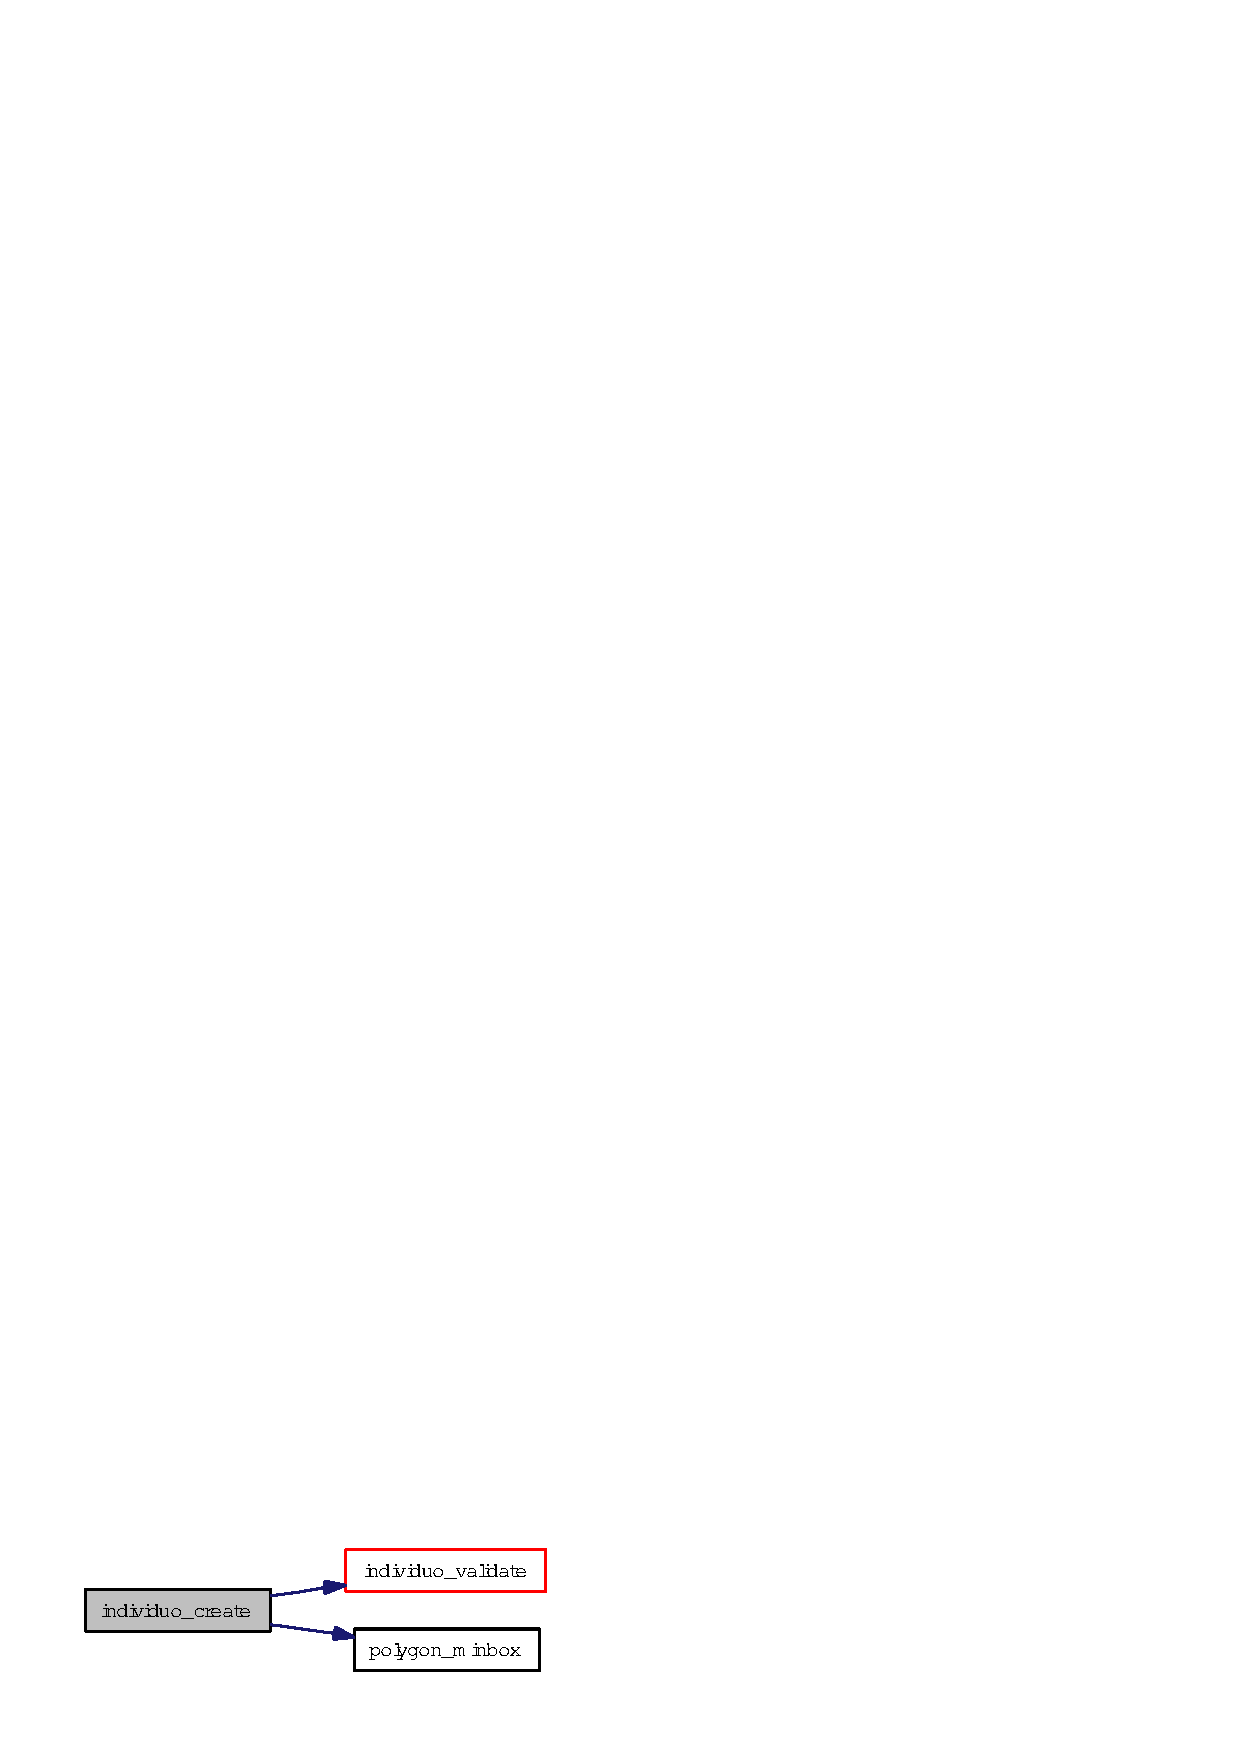
\includegraphics[width=133pt]{group__genetic_gf4e60223d27c85a5f6166e35ecafe641_gf4e60223d27c85a5f6166e35ecafe641_cgraph}
\end{center}
\end{figure}


Here is the caller graph for this function:\begin{figure}[H]
\begin{center}
\leavevmode
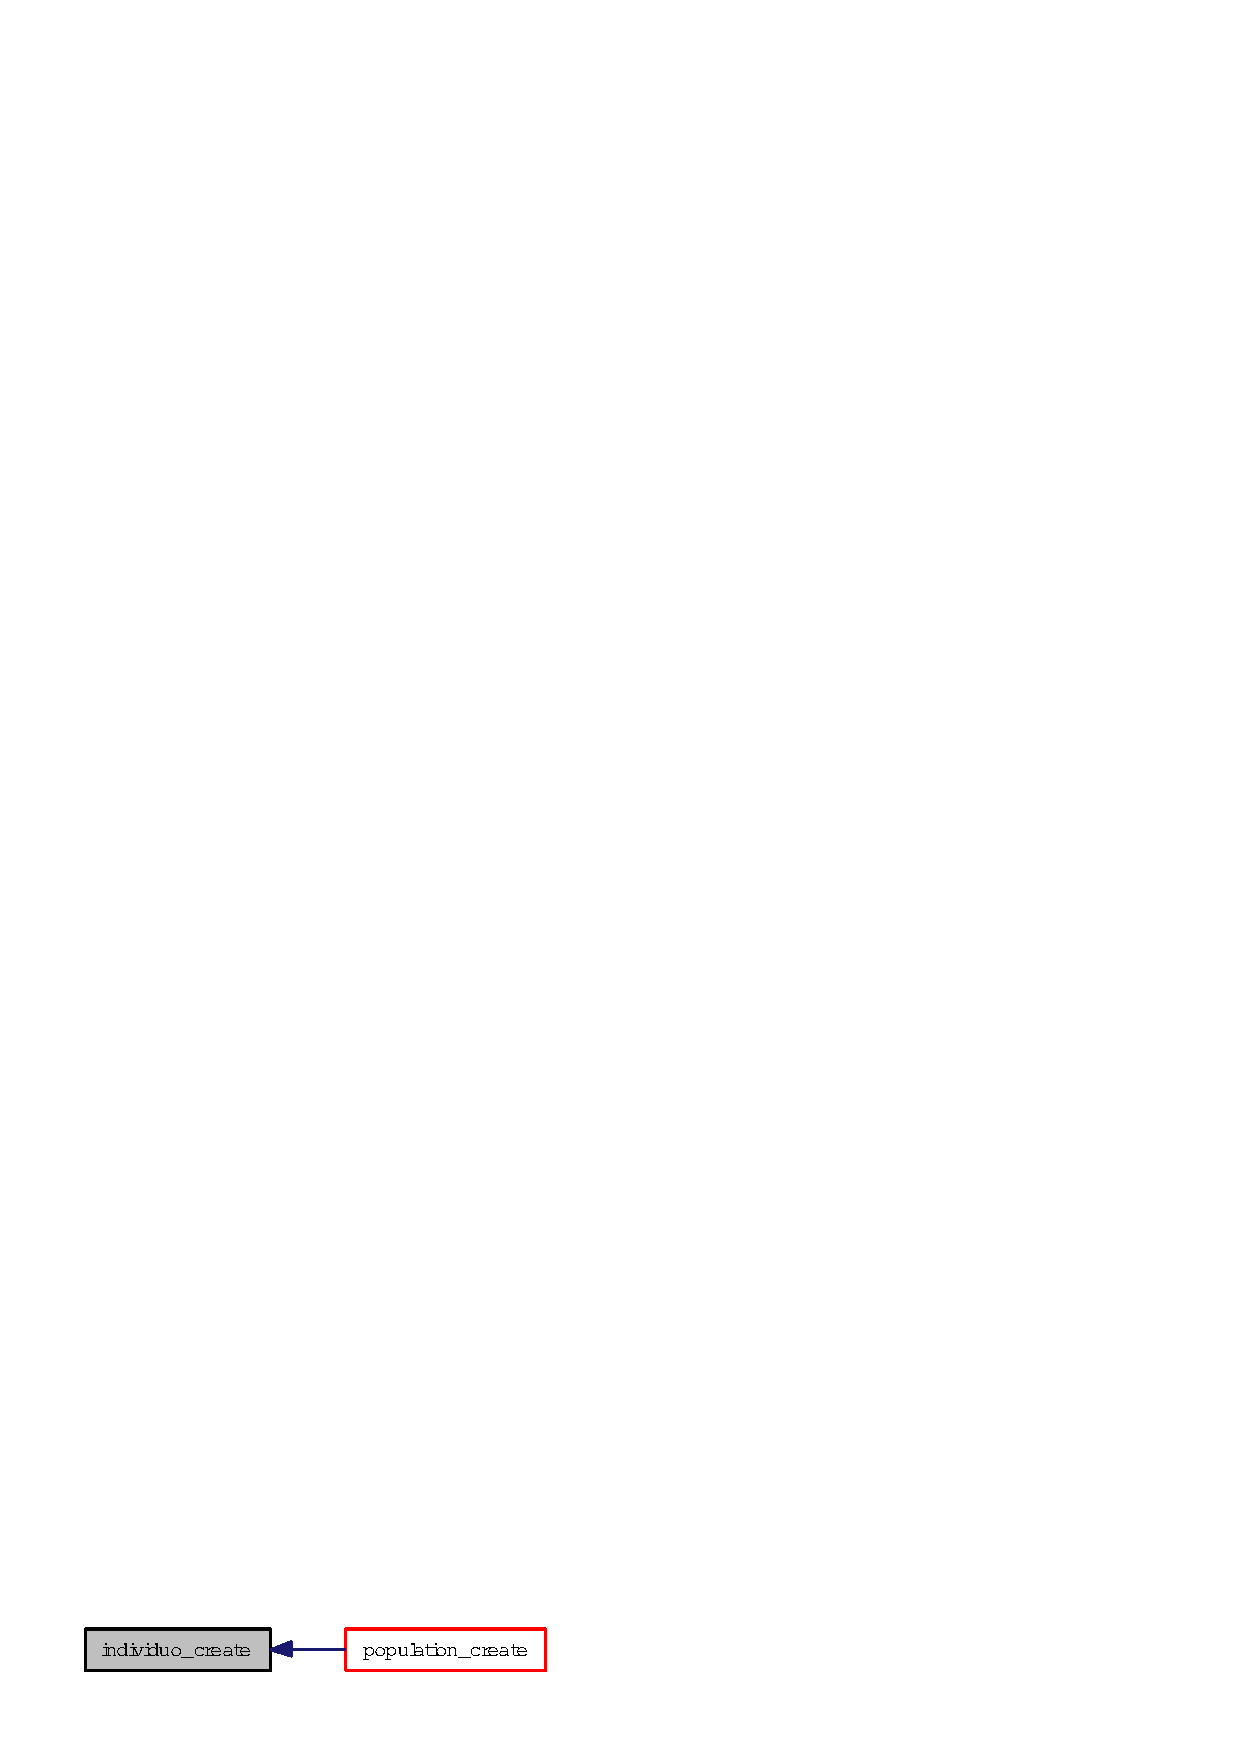
\includegraphics[width=133pt]{group__genetic_gf4e60223d27c85a5f6166e35ecafe641_gf4e60223d27c85a5f6166e35ecafe641_icgraph}
\end{center}
\end{figure}
\hypertarget{group__genetic_gf152bd4602acec2166cc4b91e8c8919a_gf152bd4602acec2166cc4b91e8c8919a}{
\index{genetic@{genetic}!individuo_fitness@{individuo\_\-fitness}}
\index{individuo_fitness@{individuo\_\-fitness}!genetic@{genetic}}
\subsubsection[individuo\_\-fitness]{\setlength{\rightskip}{0pt plus 5cm}float individuo\_\-fitness (\hyperlink{struct__individuo}{individuo} $\ast$ {\em ind})}}
\label{group__genetic_gf152bd4602acec2166cc4b91e8c8919a_gf152bd4602acec2166cc4b91e8c8919a}


\begin{Desc}
\item[\hyperlink{todo__todo000002}{Tareas Pendientes}]No es necesario recalcular el fitness de un individuo si este no ha cambiado \end{Desc}


Definici\'{o}n en la l\'{\i}nea 26 del archivo individuo.c.

\begin{Code}\begin{verbatim}27 {
28     int i,j,cont;
29 
30     polygon_holes temp;
31 
32     temp.p = &(ind->ambiente->plantilla);
33 
34     temp.h = (polygon*) malloc(sizeof(polygon)*(ind->ngenes+ind->ambiente->nhuecos));
35 
36     temp.nholes = ind->ngenes+ind->ambiente->nhuecos;
37 
38     for (i=0,cont=0;i<ind->ambiente->nhuecos;i++)
39     {
40         temp.h[cont].nvertices = ind->ambiente->huecos[i].nvertices;
41         temp.h[cont].v=(point*) malloc(sizeof(point)*temp.h[i].nvertices);
42 
43         for (j=0;j<temp.h[cont].nvertices;j++)
44         {
45             temp.h[cont].v[j].x=ind->ambiente->huecos[i].v[j].x;
46             temp.h[cont].v[j].y=ind->ambiente->huecos[i].v[j].y;
47         }
48         cont++;
49     }
50     for (i=0;i<ind->ngenes;i++)
51     {
52         temp.h[cont].nvertices = ind->ambiente->patrones[ind->posgen[i].id].nvertices;
53         temp.h[cont].v = (point*) malloc(sizeof(point)*temp.h[cont].nvertices);
54         for (j=0;j<temp.h[cont].nvertices;j++)
55         {
56             temp.h[cont].v[j].x=ind->ambiente->patrones[ind->posgen[i].id].v[j].x;
57             temp.h[cont].v[j].y=ind->ambiente->patrones[ind->posgen[i].id].v[j].y;
58         }
59         polygon_rotate(&(temp.h[cont]),ind->posgen[i].t);
60         polygon_translate(&(temp.h[cont]),ind->posgen[i].x, ind->posgen[i].y);
61         cont++;
62     }
63 
64     ind->fitness = polygonholes_volumen(&temp)/(ind->ambiente->volumen);
65 
66     ind->areautil = polygonholes_area(&temp);
67 
68     for (i=0;i<temp.nholes;i++)
69     {
70         free(temp.h[i].v);
71     }
72     free (temp.h);
73 
74     return (ind->fitness);
75 }
\end{verbatim}\end{Code}




Gr\'{a}fico de llamadas para esta funci\'{o}n:\begin{figure}[H]
\begin{center}
\leavevmode
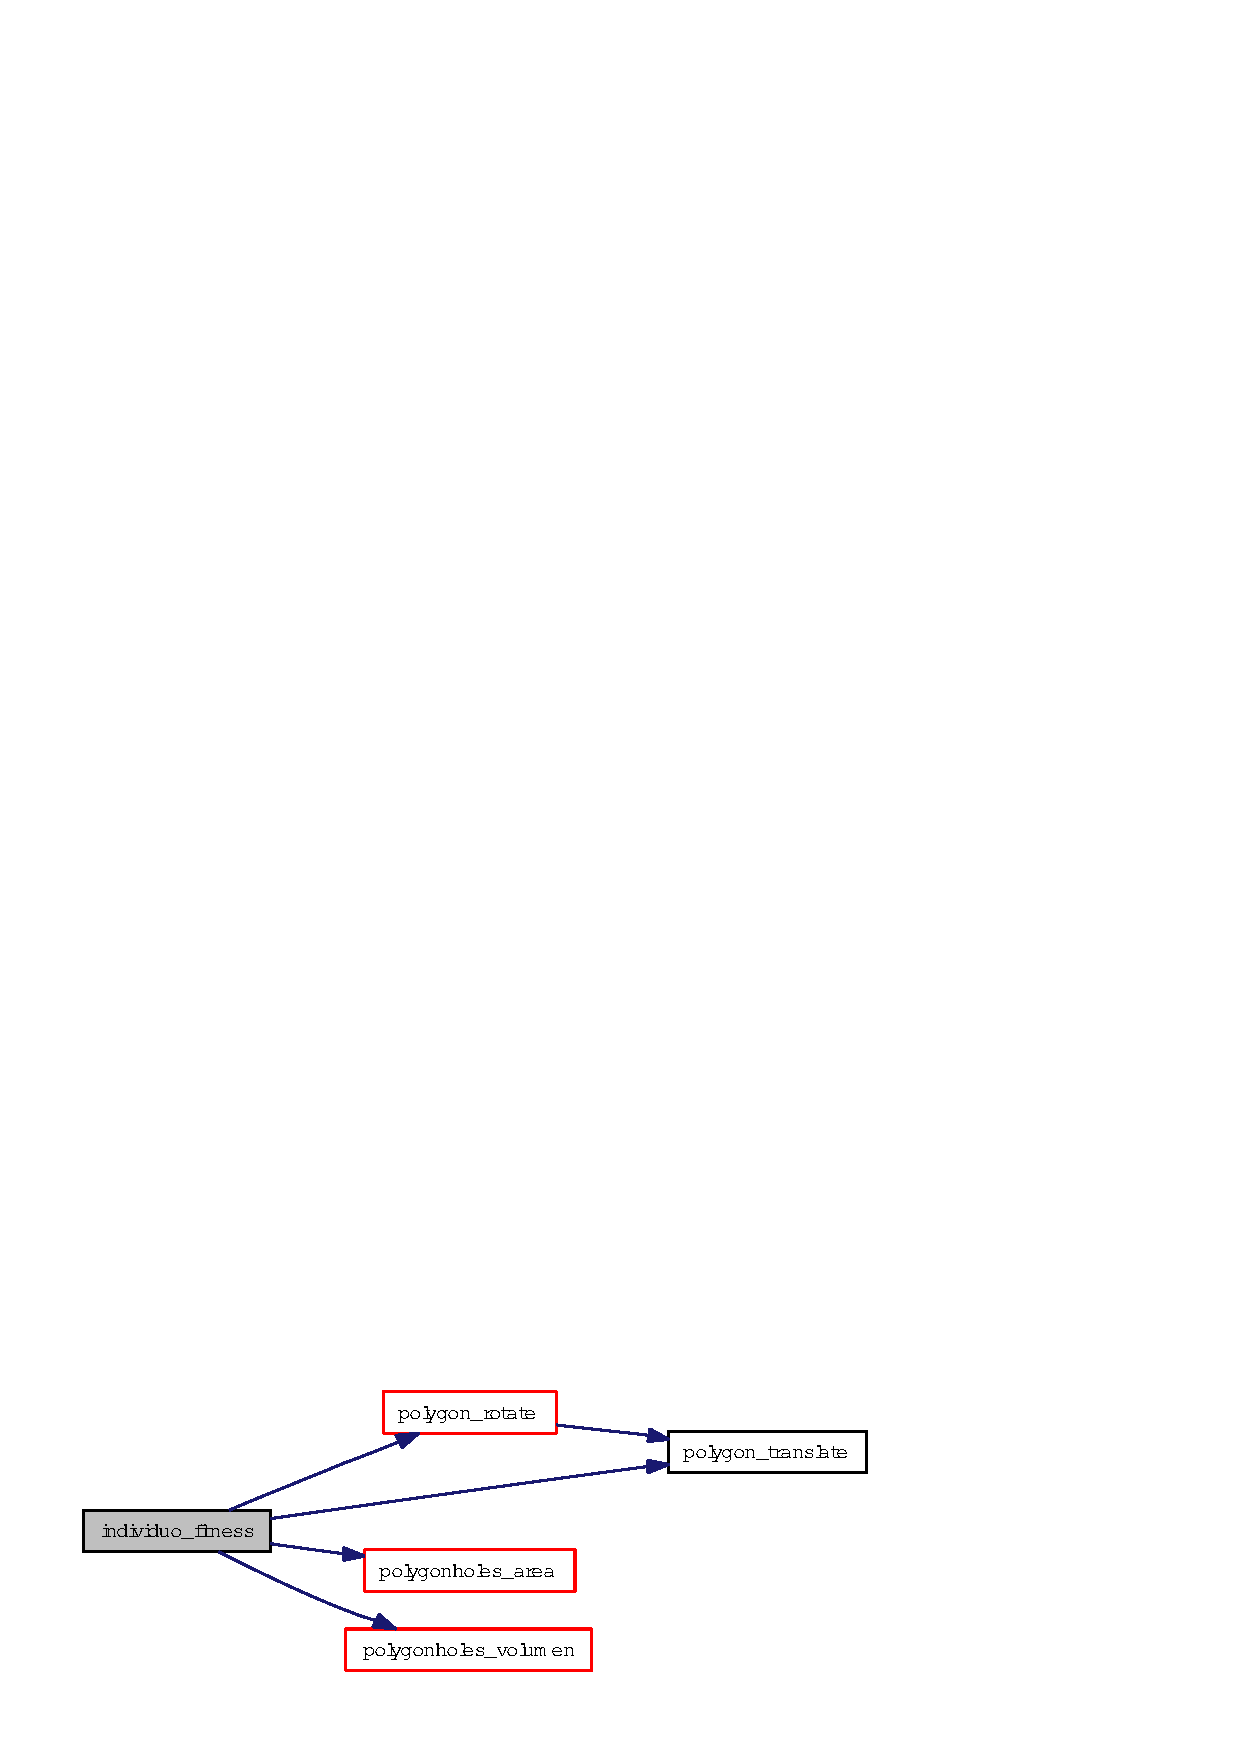
\includegraphics[width=210pt]{group__genetic_gf152bd4602acec2166cc4b91e8c8919a_gf152bd4602acec2166cc4b91e8c8919a_cgraph}
\end{center}
\end{figure}
\hypertarget{group__genetic_g05b6d3d7a4be17c9cbf479f424edd01b_g05b6d3d7a4be17c9cbf479f424edd01b}{
\index{genetic@{genetic}!individuo_mutate@{individuo\_\-mutate}}
\index{individuo_mutate@{individuo\_\-mutate}!genetic@{genetic}}
\subsubsection[individuo\_\-mutate]{\setlength{\rightskip}{0pt plus 5cm}void individuo\_\-mutate (\hyperlink{struct__individuo}{individuo} $\ast$ {\em ind})}}
\label{group__genetic_g05b6d3d7a4be17c9cbf479f424edd01b_g05b6d3d7a4be17c9cbf479f424edd01b}


Esta funcion modifica un individuo aleatoriamente.

\begin{Desc}
\item[Par\'{a}metros:]
\begin{description}
\item[\mbox{$\leftrightarrow$} {\em ind}]Individuo \end{description}
\end{Desc}


Definici\'{o}n en la l\'{\i}nea 113 del archivo individuo.c.

\begin{Code}\begin{verbatim}114 {
115     int i;
116     for (i=0;i<ind->ngenes;i++){
117         ind->posgen[i].x += (rand()%4)-2;
118         ind->posgen[i].y += (rand()%4)-2;
119         ind->posgen[i].t += ((rand()%100)-50)/100.0;
120     }
121 };
\end{verbatim}\end{Code}


\hypertarget{group__genetic_g18105662f4835e24cf3b8fc40ed63b33_g18105662f4835e24cf3b8fc40ed63b33}{
\index{genetic@{genetic}!individuo_procreate@{individuo\_\-procreate}}
\index{individuo_procreate@{individuo\_\-procreate}!genetic@{genetic}}
\subsubsection[individuo\_\-procreate]{\setlength{\rightskip}{0pt plus 5cm}void individuo\_\-procreate (\hyperlink{struct__individuo}{individuo} $\ast$ {\em p}, \hyperlink{struct__individuo}{individuo} $\ast$ {\em m}, \hyperlink{struct__individuo}{individuo} $\ast$ {\em ind})}}
\label{group__genetic_g18105662f4835e24cf3b8fc40ed63b33_g18105662f4835e24cf3b8fc40ed63b33}


Esta funcion crea un nuevo individuo partiendo de los individuos padres. La mescla se hace de la siguiente manera, se toman los patrones del padre y luego los patrones de la madre si ya no estan ya colocados, si hay patrones comunes de forma cuasi aleatoria se escoge cual de las posiciones del patron es heredada.

\begin{Desc}
\item[Par\'{a}metros:]
\begin{description}
\item[\mbox{$\leftarrow$} {\em p}]Individuo padre \item[\mbox{$\leftarrow$} {\em m}]Individuo madre \item[\mbox{$\rightarrow$} {\em ind}]Nuevo individuo \end{description}
\end{Desc}


Definici\'{o}n en la l\'{\i}nea 121 del archivo individuo.c.\hypertarget{group__genetic_gf80cc38ea4d590f6c45215f770d63778_gf80cc38ea4d590f6c45215f770d63778}{
\index{genetic@{genetic}!individuo_validate@{individuo\_\-validate}}
\index{individuo_validate@{individuo\_\-validate}!genetic@{genetic}}
\subsubsection[individuo\_\-validate]{\setlength{\rightskip}{0pt plus 5cm}bool individuo\_\-validate (\hyperlink{struct__individuo}{individuo} $\ast$ {\em ind})}}
\label{group__genetic_gf80cc38ea4d590f6c45215f770d63778_gf80cc38ea4d590f6c45215f770d63778}


Esta funcion identifica si un individuo es una solucion validad, esto es verdadero si se cumplen las siguientes condiciones:\begin{itemize}
\item No se repite ningun patron dentro de la solucion\item Todos los patrones estan dentro de la plantilla\item Ningun patron se solapa con la plantilla, huecos u otro patron En caso contrario el individuo no es valido.\end{itemize}


\begin{Desc}
\item[Par\'{a}metros:]
\begin{description}
\item[\mbox{$\leftarrow$} {\em ind}]Individuo a validar \end{description}
\end{Desc}
\begin{Desc}
\item[Devuelve:]Verdadero si es un individuo valido, falso en caso contrario. \end{Desc}


Definici\'{o}n en la l\'{\i}nea 190 del archivo individuo.c.

\begin{Code}\begin{verbatim}191 {
192     bool valido = true;
193     int i,j;
194     polygon_holes ph;
195     polygon *pat;
196 
197     for (i=0;i<ind->ngenes-1 && valido;i++)
198     {
199         for (j=i+1;j<ind->ngenes && valido;j++)
200         {
201             if (ind->posgen[i].id == ind->posgen[j].id)
202                 valido = false;
203         }
204     }
205 
206     ph.p = &(ind->ambiente->plantilla);
207     ph.nholes = ind->ambiente->nhuecos;
208     ph.h = (polygon*) malloc(sizeof(polygon)*ph.nholes);
209 
210     for (i=0;i<ph.nholes;i++)
211     {
212         ph.h[i].nvertices = ind->ambiente->huecos[i].nvertices;
213         ph.h[i].v=(point*) malloc(sizeof(point)*ph.h[i].nvertices);
214 
215         for (j=0;j<ph.h[i].nvertices;j++)
216         {
217             ph.h[i].v[j].x=ind->ambiente->huecos[i].v[j].x;
218             ph.h[i].v[j].y=ind->ambiente->huecos[i].v[j].y;
219         }
220     }
221 
222     pat = (polygon*) malloc(sizeof(polygon)*ind->ngenes);
223 
224     for (i=0;i<ind->ngenes;i++)
225     {
226         pat[i].nvertices = ind->ambiente->patrones[ind->posgen[i].id].nvertices;
227         pat[i].v = (point*) malloc(sizeof(point)*pat[i].nvertices);
228         for (j=0;j<pat[i].nvertices;j++)
229         {
230             pat[i].v[j].x=ind->ambiente->patrones[ind->posgen[i].id].v[j].x;
231             pat[i].v[j].y=ind->ambiente->patrones[ind->posgen[i].id].v[j].y;
232         }
233         polygon_rotate(&(pat[i]),ind->posgen[i].t);
234         polygon_translate(&(pat[i]),ind->posgen[i].x, ind->posgen[i].y);
235     }
236 
237     for (i=0;i<ind->ngenes && valido;i++)
238     {
239         if(!polygonholes_polygonin(&ph, &(pat[i])))
240         {
241             valido=false;
242         }
243     }
244 
245     for (i=0;i<ind->ngenes-1 && valido;i++)
246     {
247         for (j=i+1;j<ind->ngenes && valido;j++)
248         {
249             if (polygon_overlapping(&(pat[i]),&(pat[j])))
250             {
251                 valido=false;
252             }
253         }
254     }
255 
256     for (i=0;i<ind->ngenes;i++)
257     {
258         free(pat[i].v);
259     }
260     free(pat);
261 
262     for (i=0;i<ph.nholes;i++)
263     {
264         free(ph.h[i].v);
265     }
266     free(ph.h);
267 
268     return valido;
269 }
\end{verbatim}\end{Code}




Gr\'{a}fico de llamadas para esta funci\'{o}n:\begin{figure}[H]
\begin{center}
\leavevmode
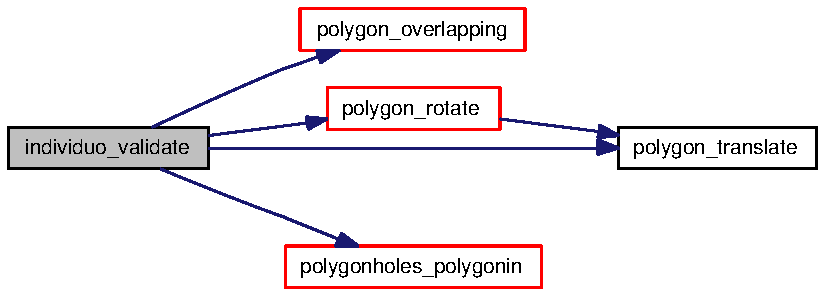
\includegraphics[width=216pt]{group__genetic_gf80cc38ea4d590f6c45215f770d63778_gf80cc38ea4d590f6c45215f770d63778_cgraph}
\end{center}
\end{figure}


Here is the caller graph for this function:\begin{figure}[H]
\begin{center}
\leavevmode
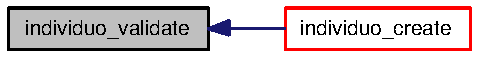
\includegraphics[width=133pt]{group__genetic_gf80cc38ea4d590f6c45215f770d63778_gf80cc38ea4d590f6c45215f770d63778_icgraph}
\end{center}
\end{figure}
\hypertarget{group__genetic_g6fed4910dd1f6172bb5a4e35a97bbe56_g6fed4910dd1f6172bb5a4e35a97bbe56}{
\index{genetic@{genetic}!leer_archivo@{leer\_\-archivo}}
\index{leer_archivo@{leer\_\-archivo}!genetic@{genetic}}
\subsubsection[leer\_\-archivo]{\setlength{\rightskip}{0pt plus 5cm}\hyperlink{struct__genesting}{genesting} $\ast$ leer\_\-archivo (char $\ast$ {\em arc\_\-name})}}
\label{group__genetic_g6fed4910dd1f6172bb5a4e35a97bbe56_g6fed4910dd1f6172bb5a4e35a97bbe56}


\begin{Desc}
\item[\hyperlink{todo__todo000001}{Tareas Pendientes}]Documentar como es la estructura leida por el programa. \end{Desc}


Definici\'{o}n en la l\'{\i}nea 25 del archivo genesting.c.

\begin{Code}\begin{verbatim}26 {
27     FILE* arc;
28     genesting *g;
29     int npoly;
30     int i,j;
31 
32     g =(genesting*) malloc (sizeof(genesting));
33 
34     arc=fopen(arc_name,"r");
35 
36     if(arc==NULL){
37             fprintf(stderr,"No se pudo abrir el archivo\n");
38             exit(1);
39     }
40 
41     fscanf(arc,"%i",&npoly);
42 
43     g->nhuecos =0;
44     g->npatrones =0;
45 
46     g->huecos=(polygon*) malloc(sizeof(polygon)*npoly-1);
47     g->patrones=(polygon*) malloc(sizeof(polygon)*npoly-1);
48 
49     for (i=0;i<npoly;i++)
50     {
51         int nvert,tipo;
52 
53         polygon *p=NULL;
54         fscanf(arc,"%i %i",&nvert,&tipo);
55         switch(tipo)
56         {
57             case 1:
58             p=&(g->plantilla);
59             break;
60             case 2:
61             p=&(g->patrones[g->npatrones++]);
62             break;
63             case 3:
64             p=&(g->huecos[g->nhuecos++]);
65             break;
66         }
67         p->nvertices = nvert;
68         p->v=(point*) malloc(sizeof(point)*nvert);
69         for (j=0;j<nvert;j++)
70         {
71             fscanf(arc,"%f %f",&(p->v[j].x),&(p->v[j].y));
72         }
73     }
74     g->huecos=(polygon*) realloc(g->huecos,sizeof(polygon)*g->nhuecos);
75     g->patrones=(polygon*) realloc(g->patrones,sizeof(polygon)*g->npatrones);
76 
77     fclose(arc);
78 
79     return g;
80 }
\end{verbatim}\end{Code}




Here is the caller graph for this function:\begin{figure}[H]
\begin{center}
\leavevmode
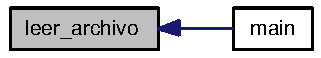
\includegraphics[width=95pt]{group__genetic_g6fed4910dd1f6172bb5a4e35a97bbe56_g6fed4910dd1f6172bb5a4e35a97bbe56_icgraph}
\end{center}
\end{figure}
\hypertarget{group__genetic_gc7ba874876f18abab66f0a42f32b98cc_gc7ba874876f18abab66f0a42f32b98cc}{
\index{genetic@{genetic}!population_create@{population\_\-create}}
\index{population_create@{population\_\-create}!genetic@{genetic}}
\subsubsection[population\_\-create]{\setlength{\rightskip}{0pt plus 5cm}void population\_\-create (\hyperlink{struct__population}{population} $\ast$ {\em p}, \hyperlink{struct__genesting}{genesting} $\ast$ {\em g}, int {\em n})}}
\label{group__genetic_gc7ba874876f18abab66f0a42f32b98cc_gc7ba874876f18abab66f0a42f32b98cc}


Esta funcion crea una poblacion inicial de soluciones.

\begin{Desc}
\item[Par\'{a}metros:]
\begin{description}
\item[\mbox{$\rightarrow$} {\em p}]Poblacion \item[\mbox{$\leftarrow$} {\em g}]Genesting \item[\mbox{$\leftarrow$} {\em n}]Numero de elementos de la poblacion \end{description}
\end{Desc}


Definici\'{o}n en la l\'{\i}nea 23 del archivo population.c.

\begin{Code}\begin{verbatim}23                                                           {
24     int i;
25     p->ambiente=g;
26     p->nindividuos=n;
27     p->individuos = (individuo*) malloc(sizeof(individuo)*p->nindividuos);
28 
29     for (i=0;i<p->nindividuos;i++){
30             individuo_create(p->ambiente,&(p->individuos[i]));
31     }
32 };
\end{verbatim}\end{Code}




Gr\'{a}fico de llamadas para esta funci\'{o}n:\begin{figure}[H]
\begin{center}
\leavevmode
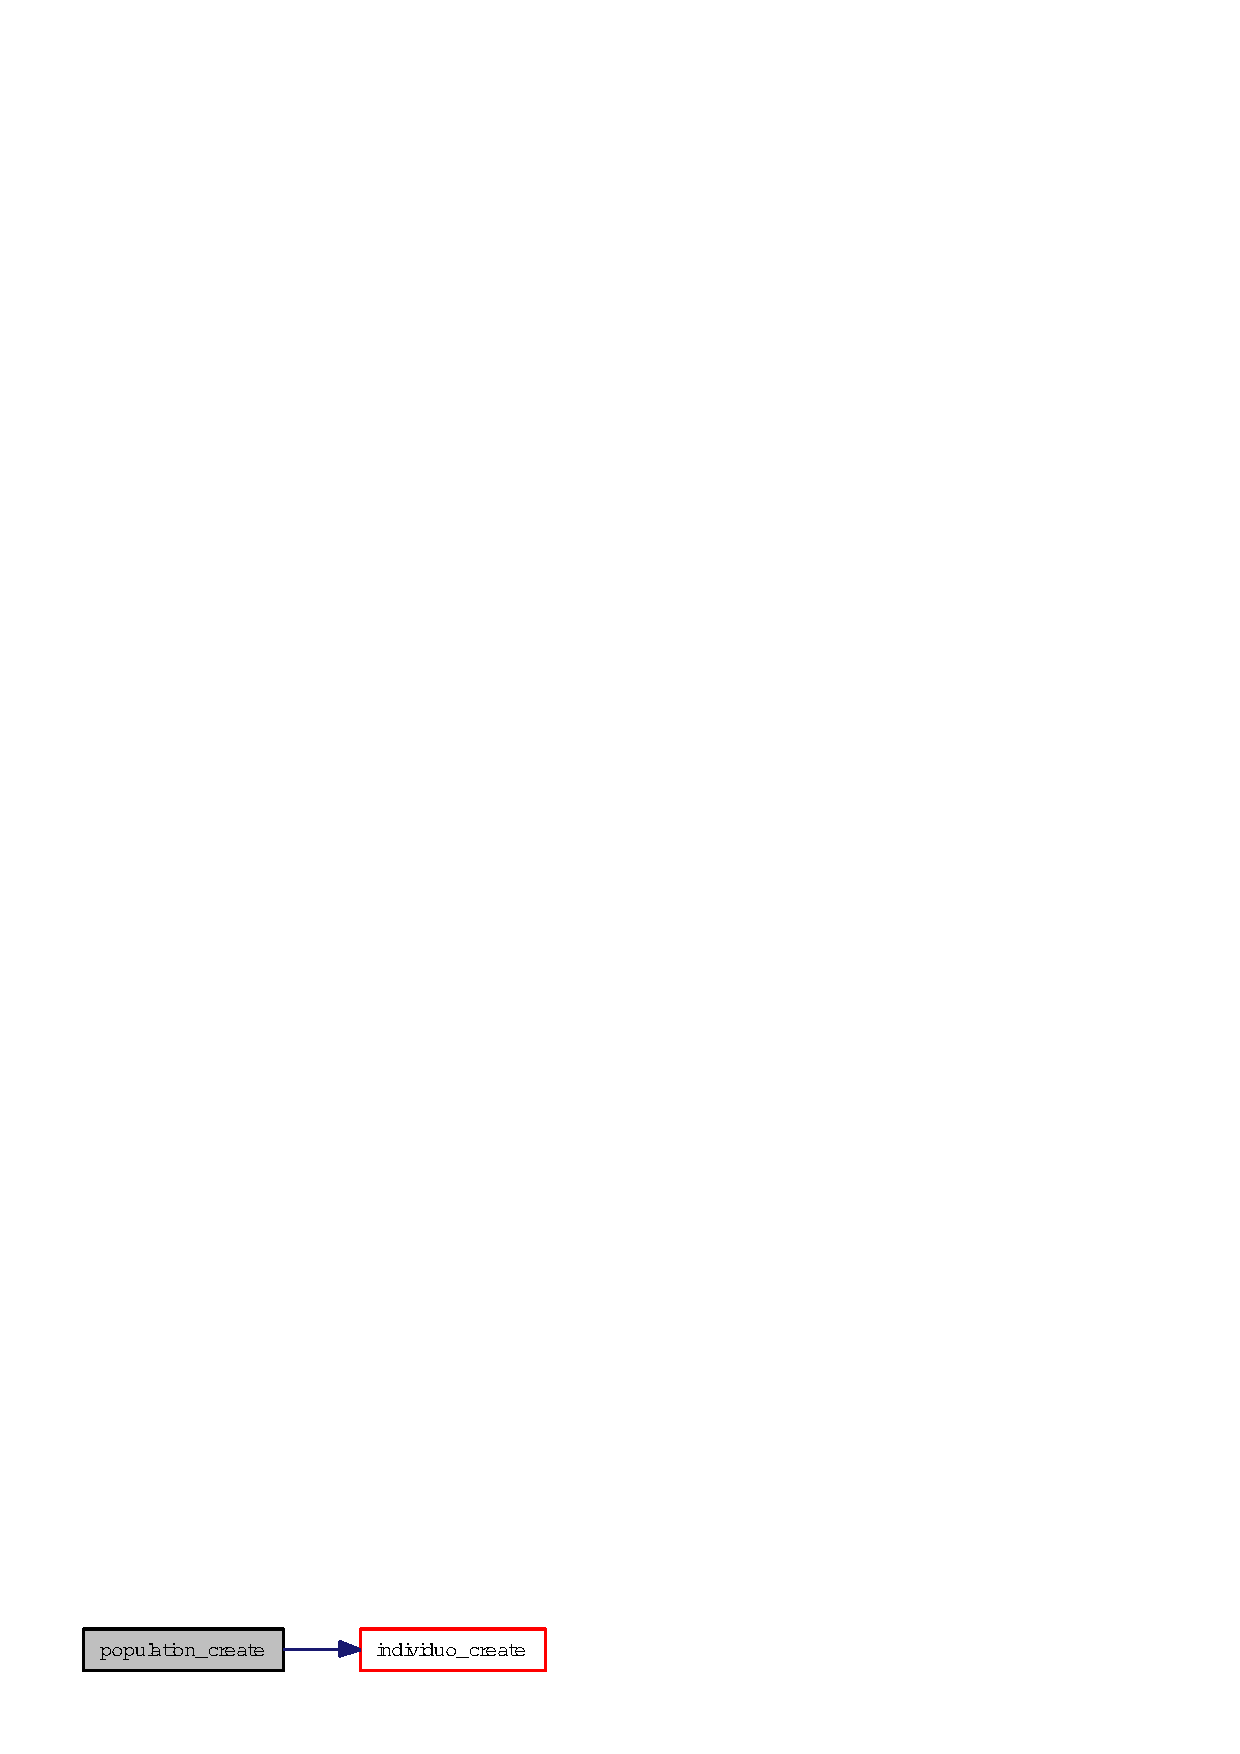
\includegraphics[width=133pt]{group__genetic_gc7ba874876f18abab66f0a42f32b98cc_gc7ba874876f18abab66f0a42f32b98cc_cgraph}
\end{center}
\end{figure}


Here is the caller graph for this function:\begin{figure}[H]
\begin{center}
\leavevmode
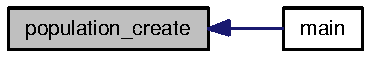
\includegraphics[width=107pt]{group__genetic_gc7ba874876f18abab66f0a42f32b98cc_gc7ba874876f18abab66f0a42f32b98cc_icgraph}
\end{center}
\end{figure}
\hypertarget{group__genetic_g229293c432c5ef4f70b1ee94c109bb1a_g229293c432c5ef4f70b1ee94c109bb1a}{
\index{genetic@{genetic}!population_evaluate@{population\_\-evaluate}}
\index{population_evaluate@{population\_\-evaluate}!genetic@{genetic}}
\subsubsection[population\_\-evaluate]{\setlength{\rightskip}{0pt plus 5cm}void population\_\-evaluate (\hyperlink{struct__population}{population} $\ast$ {\em p})}}
\label{group__genetic_g229293c432c5ef4f70b1ee94c109bb1a_g229293c432c5ef4f70b1ee94c109bb1a}


Evalua una poblacion, para esto calcula todos los fitness, y ordena los individuos segun su fitness

\begin{Desc}
\item[Par\'{a}metros:]
\begin{description}
\item[\mbox{$\leftrightarrow$} {\em p}]Poblacion \end{description}
\end{Desc}


Definici\'{o}n en la l\'{\i}nea 32 del archivo population.c.

Here is the caller graph for this function:\begin{figure}[H]
\begin{center}
\leavevmode
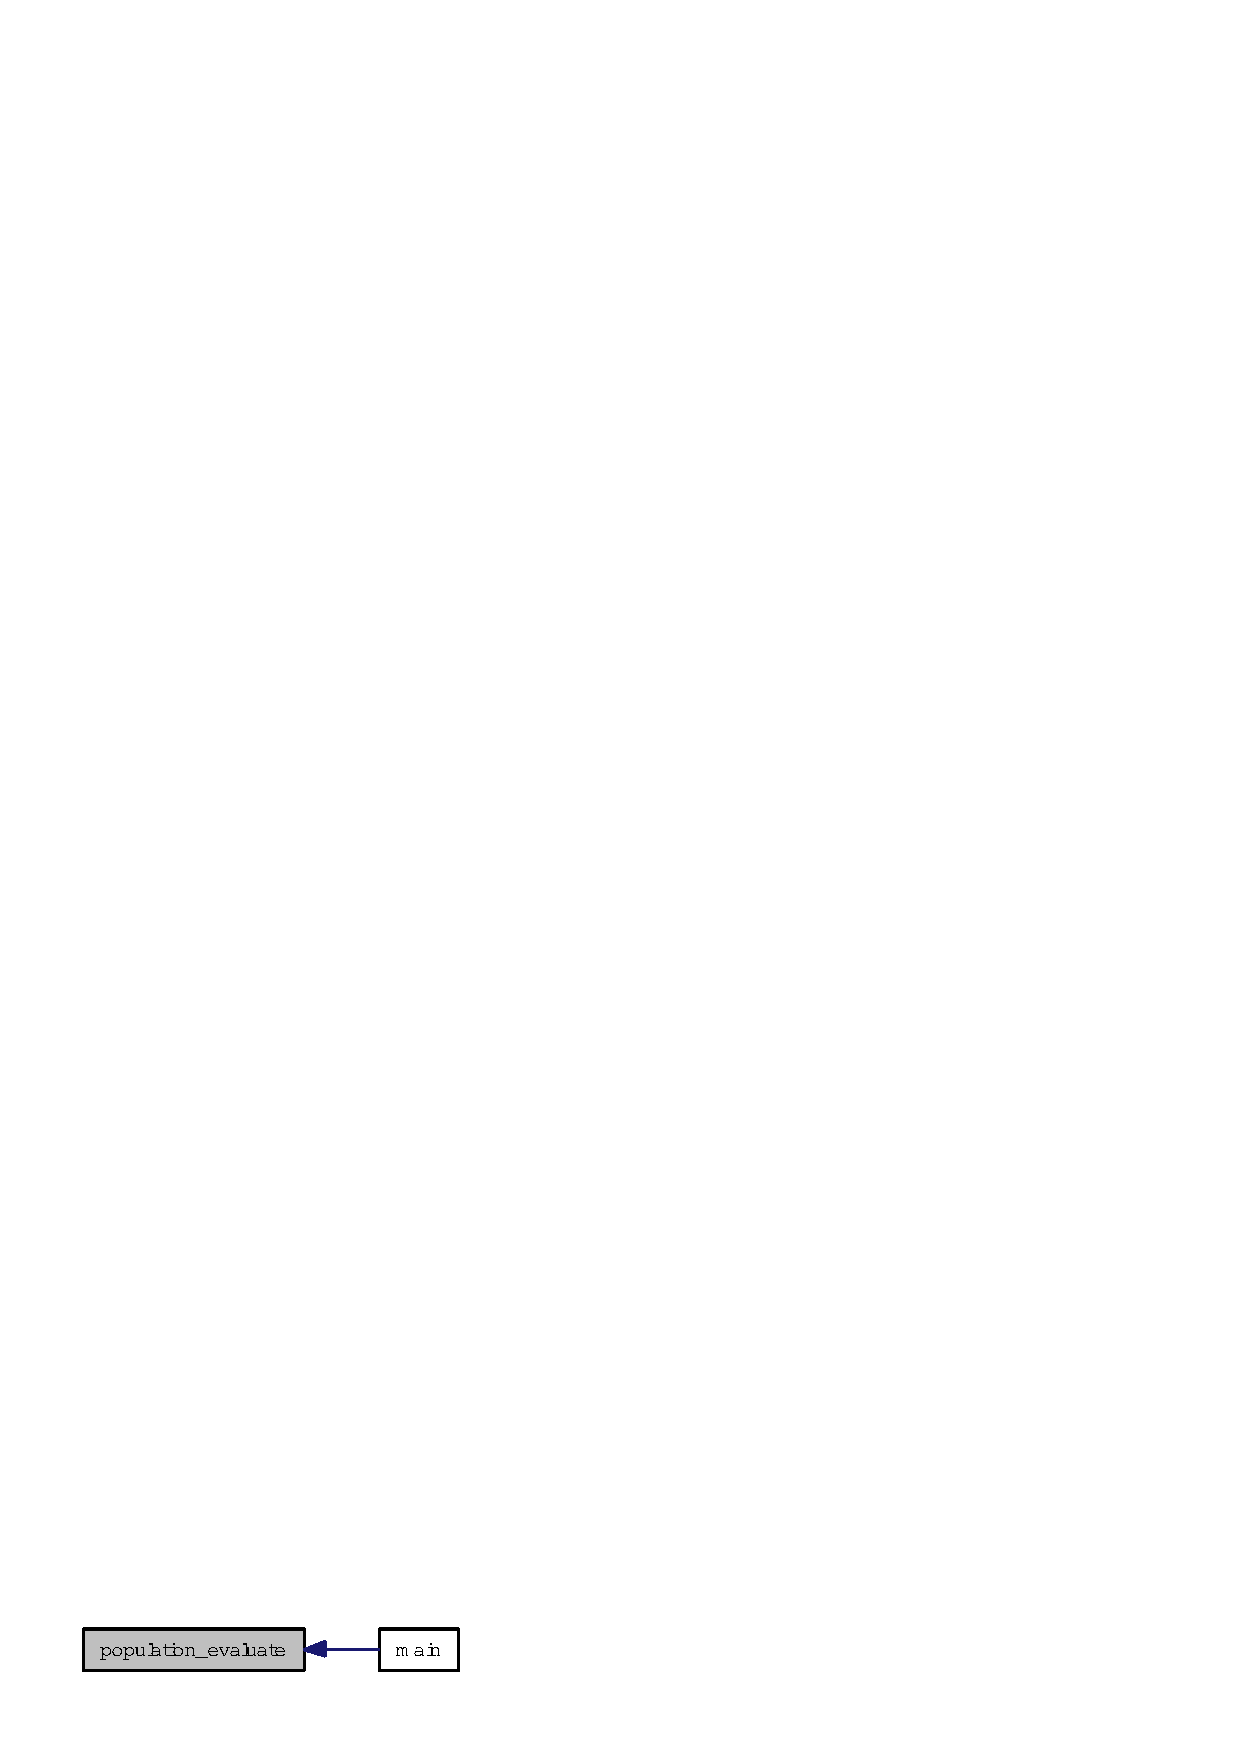
\includegraphics[width=112pt]{group__genetic_g229293c432c5ef4f70b1ee94c109bb1a_g229293c432c5ef4f70b1ee94c109bb1a_icgraph}
\end{center}
\end{figure}
\hypertarget{group__genetic_g5b3202f02e14d7fb3eb1f729d1250243_g5b3202f02e14d7fb3eb1f729d1250243}{
\index{genetic@{genetic}!population_generation@{population\_\-generation}}
\index{population_generation@{population\_\-generation}!genetic@{genetic}}
\subsubsection[population\_\-generation]{\setlength{\rightskip}{0pt plus 5cm}void population\_\-generation (\hyperlink{struct__population}{population} $\ast$ {\em p})}}
\label{group__genetic_g5b3202f02e14d7fb3eb1f729d1250243_g5b3202f02e14d7fb3eb1f729d1250243}


Crea una nueva poblacion, dividiendo la exitente en tres grupos, dejando el primer grupo intacto, el segundo lo muta, y el tercero es un cruce de los 2 primeros \begin{Desc}
\item[Par\'{a}metros:]
\begin{description}
\item[\mbox{$\leftrightarrow$} {\em p}]Poblacion \end{description}
\end{Desc}


Definici\'{o}n en la l\'{\i}nea 47 del archivo population.c.

Here is the caller graph for this function:\begin{figure}[H]
\begin{center}
\leavevmode
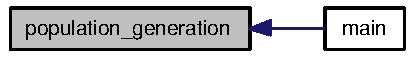
\includegraphics[width=117pt]{group__genetic_g5b3202f02e14d7fb3eb1f729d1250243_g5b3202f02e14d7fb3eb1f729d1250243_icgraph}
\end{center}
\end{figure}
